% =====================================================================
% RESULTADOS E CONCLUSÃO
% Todos os números vêm dos treinos e avaliações rodados neste PC
% (30/09 e 01/10/2026), semente 0.
% Preâmbulo: \usepackage{graphicx}, \usepackage{amsmath}
% Figuras: copie a pasta "graficos" (curvas.png e sequencia_sac.png)
% para junto do seu .tex, ou ajuste o caminho no \includegraphics.
% =====================================================================

\section{Resultados}

Os resultados a seguir correspondem a uma execução de cada configuração (semente 0). Durante o treinamento, os agentes foram avaliados a cada 10.000 passos em 20 episódios com a política determinística. Ao final, o melhor modelo de cada configuração foi avaliado em 100 episódios, com as posições da caixa definidas pelas sementes 1000 a 1099, as mesmas para todos os agentes.

\subsection{Curvas de aprendizado}

A Figura~\ref{fig:curvas} apresenta a evolução do retorno médio e da taxa de sucesso ao longo do treinamento. As curvas começam em 10.000 passos, que é o momento da primeira avaliação; por isso, o primeiro ponto já reflete o que cada agente aprendeu nesse intervalo, e não o comportamento sem treino.

\begin{figure}[htb]
    \centering
    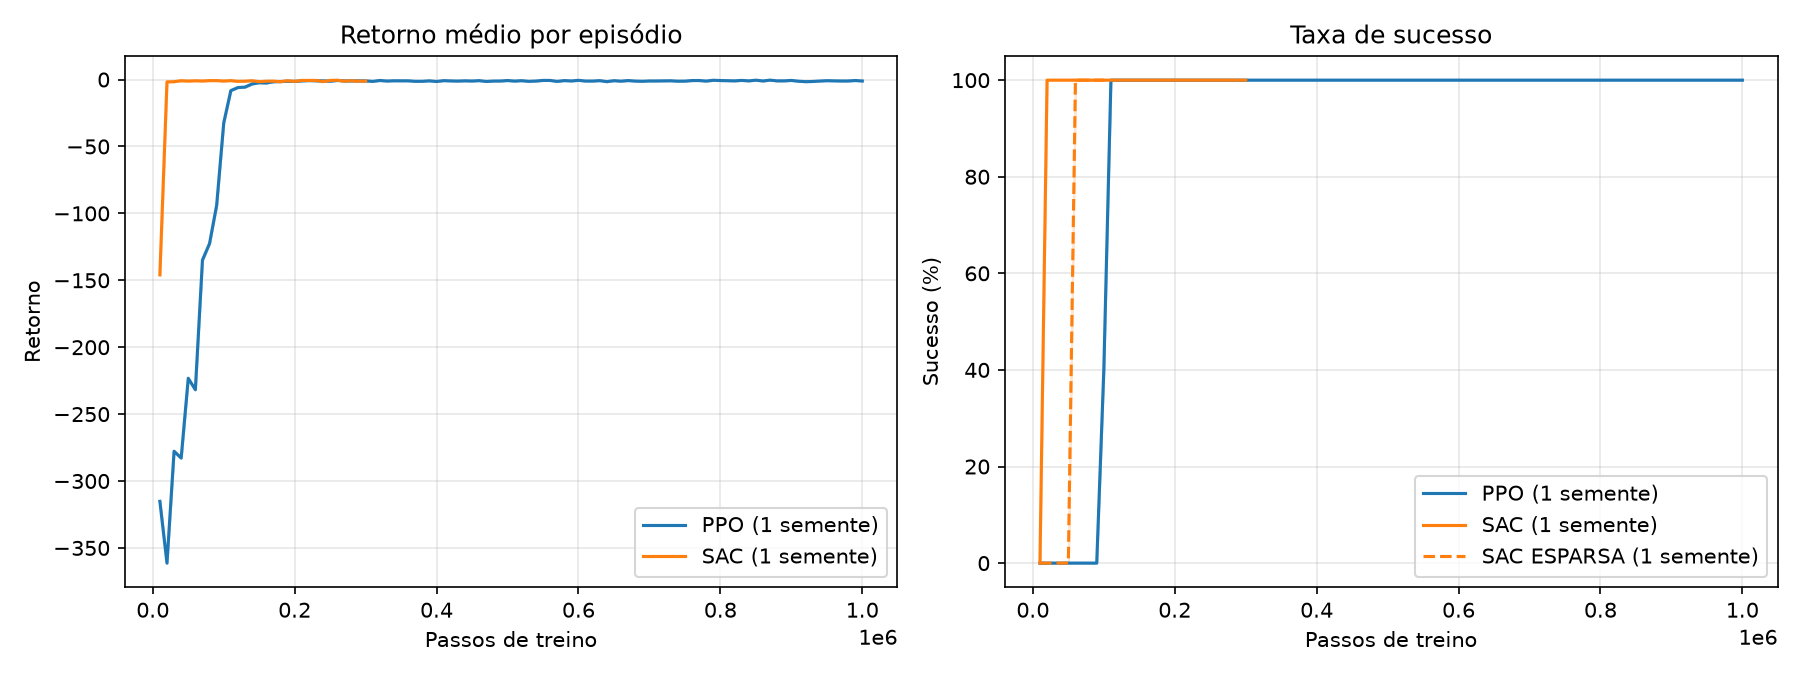
\includegraphics[width=\textwidth]{graficos/curvas.png}
    \caption{Retorno médio por episódio (esquerda) e taxa de sucesso (direita) em função dos passos de treinamento. A linha tracejada corresponde ao SAC treinado com recompensa esparsa, mostrado apenas na taxa de sucesso por ter retorno em outra escala.}
    \label{fig:curvas}
\end{figure}

No SAC, o retorno médio passou de $-145{,}9$ na avaliação de 10.000 passos para $-1{,}7$ na de 20.000 passos, quando a taxa de sucesso atingiu 100\%, e permaneceu nesse patamar até o fim dos 300.000 passos. O valor de $-145{,}9$ indica que, com 10.000 passos, dos quais os 5.000 primeiros foram de ações aleatórias, o agente já agarrava a caixa em parte dos episódios, embora ainda não a elevasse até a altura-alvo: como cada passo sem a caixa custa pelo menos $-1$ e os episódios sem sucesso duram 250 passos, um agente que nunca agarrasse a caixa teria retorno inferior a $-250$.

No PPO, a evolução foi mais gradual. O retorno partiu de $-315{,}2$ com 10.000 passos, oscilou entre $-360$ e $-220$ até 60.000 passos e subiu de forma consistente a partir daí, chegando a $-32{,}4$ com 100.000 passos, quando a taxa de sucesso foi de 40\%. A partir de 110.000 passos, a taxa de sucesso chegou a 100\% e se manteve até o fim do treinamento, com 1.000.000 de passos, e o retorno se estabilizou em torno de $-1$.

\subsection{Eficiência de amostras}

A Tabela~\ref{tab:eficiencia} resume a quantidade de passos de treinamento necessária para que cada agente atingisse 100\% de sucesso nas avaliações periódicas. Como as avaliações ocorrem a cada 10.000 passos, os valores indicam o primeiro ponto avaliado em que isso ocorreu.

\begin{table}[htb]
    \centering
    \caption{Passos de treinamento até 100\% de sucesso nas avaliações}
    \label{tab:eficiencia}
    \begin{tabular}{lcc}
        \hline
        Configuração & Último ponto com 0\% & Primeiro ponto com 100\% \\
        \hline
        SAC, recompensa em etapas    & 10.000 & 20.000 \\
        PPO, recompensa em etapas    & 90.000 & 110.000 \\
        SAC, recompensa esparsa      & 50.000 & 60.000 \\
        \hline
    \end{tabular}
\end{table}

O SAC precisou de cerca de 5 vezes menos interações com o ambiente que o PPO para resolver a tarefa. Com a recompensa esparsa, o SAC também aprendeu a tarefa, mas precisou de cerca de 3 vezes mais passos do que com a recompensa em etapas.

\subsection{Desempenho final}

A Tabela~\ref{tab:final} mostra a avaliação final em 100 episódios. Para referência, foram incluídos um agente sem treinamento, que executa ações aleatórias, e o SAC com recompensa esparsa interrompido em 30.000 passos, antes de aprender a tarefa.

\begin{table}[htb]
    \centering
    \caption{Avaliação final em 100 episódios}
    \label{tab:final}
    \begin{tabular}{lccc}
        \hline
        Agente & Sucesso & Passos por episódio & Menor distância média \\
               &         &                     & até a caixa (m) \\
        \hline
        Sem treino (ações aleatórias)            & 0\%   & 250,0 & 0,399 \\
        SAC, recompensa esparsa, 30.000 passos   & 0\%   & 250,0 & 0,168 \\
        SAC, recompensa esparsa, 100.000 passos  & 100\% & 16,2  & 0,032 \\
        SAC, recompensa em etapas, 300.000 passos & 100\% & 15,3  & 0,044 \\
        PPO, recompensa em etapas, 1.000.000 passos & 100\% & 15,1  & 0,033 \\
        \hline
    \end{tabular}
\end{table}

Os dois algoritmos com recompensa em etapas obtiveram 100\% de sucesso, levando em média cerca de 15 passos para alcançar, agarrar e elevar a caixa. Os retornos médios também foram praticamente iguais: $-1{,}17 \pm 1{,}29$ para o SAC e $-1{,}14 \pm 1{,}23$ para o PPO. Assim, ao final do treinamento, não houve diferença de desempenho entre os algoritmos; a diferença está na quantidade de experiência necessária para chegar a esse resultado.

Os agentes que falharam também diferem entre si. O agente aleatório chegou, em média, a no mínimo 0,40~m da caixa, enquanto o SAC com recompensa esparsa interrompido em 30.000 passos chegou a 0,17~m. Esse agente já movia a garra na direção da caixa, mas não alcançava a distância de 0,05~m necessária para a preensão e terminava todos os episódios pelo limite de 250 passos.

\subsection{Análise qualitativa}

A Figura~\ref{fig:sequencia} mostra quadros renderizados em OpenGL de um episódio do SAC treinado. Partindo da postura inicial (a), o agente abaixa o braço em direção à caixa (b), fecha a garra ao redor dela no nono passo (c), quando a caixa muda de cor para indicar a preensão, e a eleva até a altura-alvo, marcada pela linha verde, no décimo quarto passo (d). O agente aprendeu a coordenar as três juntas simultaneamente, respeitando os seus limites angulares, em vez de movê-las uma de cada vez.

\begin{figure}[htb]
    \centering
    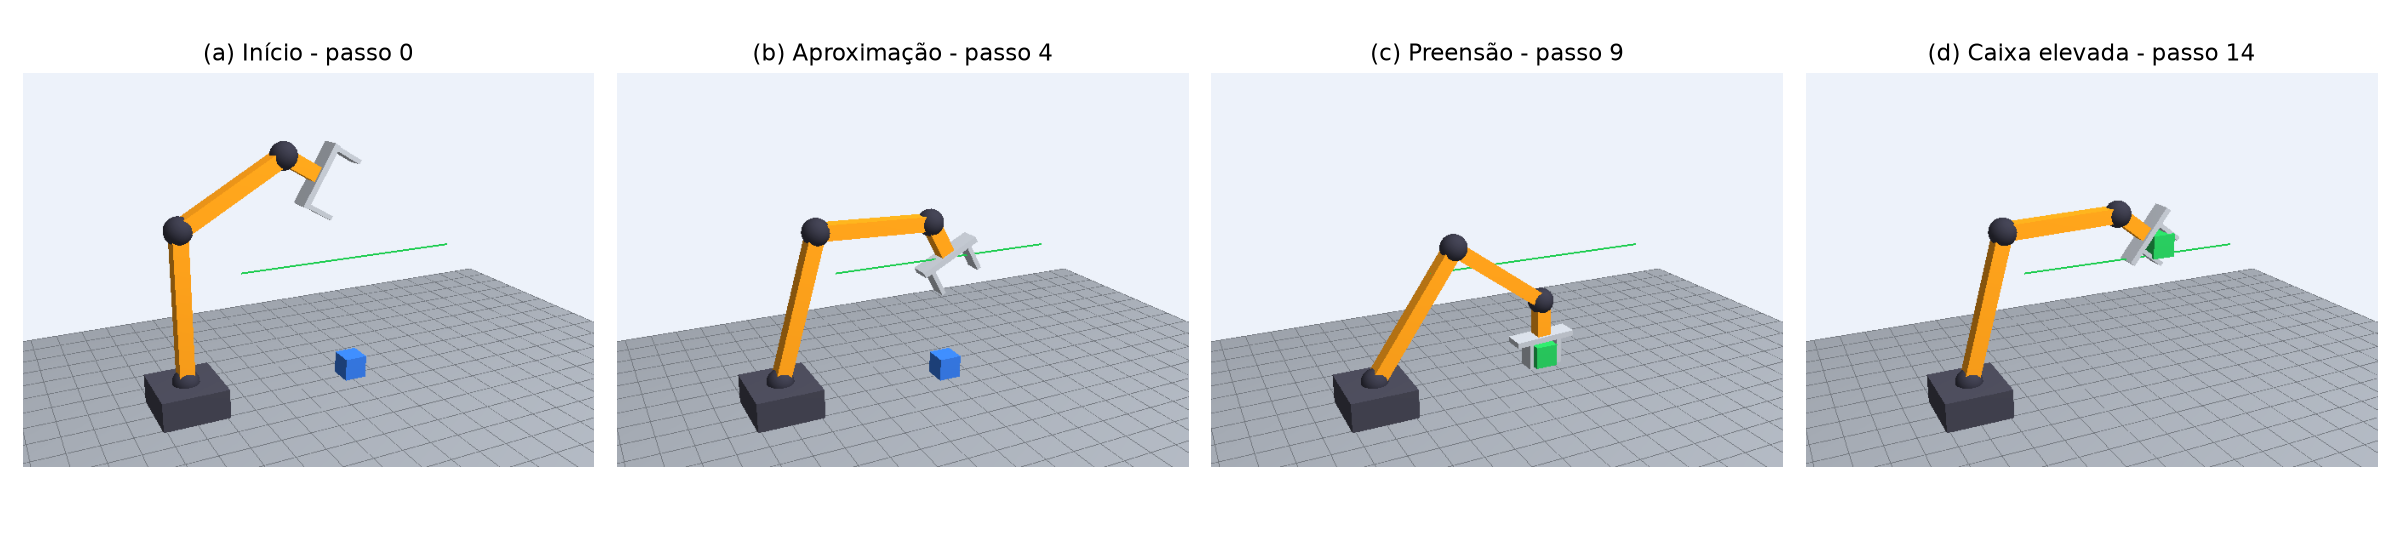
\includegraphics[width=\textwidth]{graficos/sequencia_sac.png}
    \caption{Episódio do SAC treinado, renderizado em OpenGL: (a) postura inicial; (b) aproximação; (c) preensão, com a caixa em verde indicando que está presa; (d) caixa elevada até a altura-alvo (linha verde).}
    \label{fig:sequencia}
\end{figure}

\subsection{Discussão}

A diferença na eficiência de amostras está de acordo com o funcionamento dos algoritmos. O SAC armazena todas as transições no \textit{replay buffer} e realiza uma atualização a cada passo, reaproveitando cada experiência muitas vezes, inclusive as poucas em que o braço se aproximou ou agarrou a caixa. O PPO, por ser \textit{on-policy}, utiliza cada lote de 8.192 transições em apenas 10 épocas e depois o descarta, necessitando de mais interações para acumular o mesmo aprendizado. Em contrapartida, cada passo do PPO é computacionalmente mais barato e pode ser executado em vários ambientes em paralelo. O tempo de treinamento não foi comparado, pois os treinamentos foram executados simultaneamente na mesma máquina, disputando o processador, o que tornaria a medição pouco confiável.

O experimento com recompensa esparsa mostra que a recompensa em etapas acelerou o aprendizado, mas não foi indispensável nesta tarefa. Isso se deve, em grande parte, às simplificações do ambiente: o movimento ocorre em um plano, a caixa está sempre ao alcance do braço e a preensão é considerada bem-sucedida apenas pela distância e pelo fechamento da garra. Nessas condições, a exploração aleatória inicial do SAC foi suficiente para que alguns episódios de sucesso fossem encontrados e reaproveitados.

Algumas limitações devem ser consideradas. Os resultados se baseiam em uma única semente por configuração; como o desempenho de algoritmos de aprendizado por reforço varia entre execuções, a repetição com mais sementes é necessária para confirmar as diferenças observadas. A física simplificada, sem atrito e sem forças de contato, torna a tarefa mais fácil do que em um braço real, e a granularidade de 10.000 passos entre avaliações limita a precisão com que se pode identificar o momento do aprendizado.

\section{Conclusão}

Este trabalho apresentou um ambiente de simulação de um braço robótico com garra, renderizado em OpenGL, no qual o agente aprende sozinho, por aprendizado por reforço, a alcançar, agarrar e elevar uma caixa posicionada aleatoriamente. O braço possui três juntas rotacionais com limites angulares, sem rotação completa, e é controlado por ações contínuas. A renderização por modelagem hierárquica com a pilha de matrizes do OpenGL permitiu visualizar o comportamento aprendido, enquanto a separação entre simulação e renderização permitiu treinar os agentes sem interface gráfica.

Os dois algoritmos avaliados, PPO e SAC, aprenderam a tarefa e alcançaram 100\% de sucesso em 100 episódios de teste, concluindo-a em cerca de 15 passos. O SAC, por reaproveitar as experiências armazenadas, atingiu esse desempenho com aproximadamente 20.000 passos de treinamento, contra cerca de 110.000 do PPO, o que confirma a maior eficiência de amostras dos métodos \textit{off-policy} em problemas de controle contínuo. O experimento de controle mostrou ainda que a recompensa em etapas acelerou o aprendizado em cerca de três vezes em relação à recompensa esparsa.

Como trabalhos futuros, sugerem-se: repetir os experimentos com mais sementes, para dar validade estatística à comparação; adicionar uma junta de rotação da base, tornando o movimento tridimensional; adotar um motor de física com atrito e contato, como PyBullet ou MuJoCo; usar as imagens renderizadas pelo OpenGL como entrada do agente, no lugar das coordenadas; incluir várias caixas e a tarefa de empilhá-las; e, por fim, transferir a política aprendida para um braço físico.
